\section{Детерминированный анализ}

    \subsection{Описание модели}

        Одна из вариаций модели Хасселя \cite{densityDependenceInSingleSpeciesPopulations} имеет следующую математическая запись:

        \begin{equation}
            \label{origin}
            x_{t+1} = \frac{\alpha x_t^2}{(\beta + x_t)^6}.
        \end{equation}

        В данной формуле \(x_i\) --- количество особей в поколении с номером \(i\). Параметр \(\alpha\) определяет скорость роста популяции, а параметр \(\beta\) определяет несущую способность окружающей среды.
    
        Для упрощения задачи рассмотрим частный случай. Зафиксируем параметр \(\alpha = 1\). Параметр \(\beta\) изменяется в диапазоне \([0; 0.6]\). 
        Для нахождения равновесий требуется решить следующее уравнение:  

        \[x = \frac{\alpha x^2}{(\beta + x)^6}\]
    
        \[1 = \frac{\alpha x}{(\beta + x)^6}\]

        \begin{equation}
            \label{baseEquation}
            \alpha x = (\beta + x)^6
        \end{equation}

        Построим графики функций \(y = \alpha x\) и \(y = (\beta + x)^6\). 
        
        В зависимости от значений параметра \(\beta\) уравнение (\ref{baseEquation}) может иметь ноль (при \(\beta > 0.582355932\)), один (при \(\beta \approx 0.582355932\)) или два корня (при \(\beta < 0.582355932\)). На рисунках \ref{mainIntersect}, \ref{mainTouch} и \ref{mainOver} можно увидеть все возможные варианты. При \(\beta=0.582355932\) в модели наблюдается касательная бифуркации, сопровождающаяся появлением двух равновесий.

        \begin{figure}
            \centering
            \subfloat[\(\beta = 0.57\)]{
                \label{mainIntersect}
                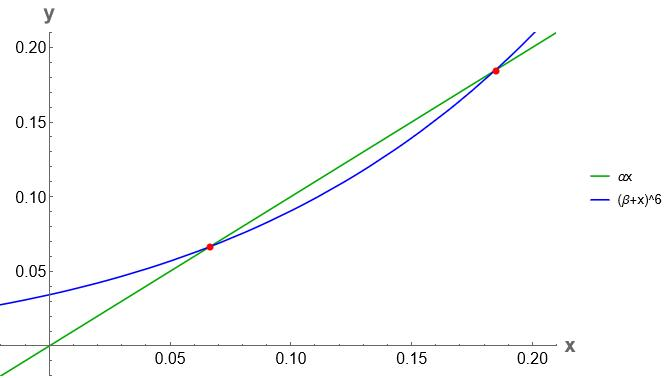
\includegraphics[width=0.77\textwidth]{images/two_intersection.jpg}
            }

            \subfloat[\(\beta \approx 0.582355932\)]{
                \label{mainTouch}
                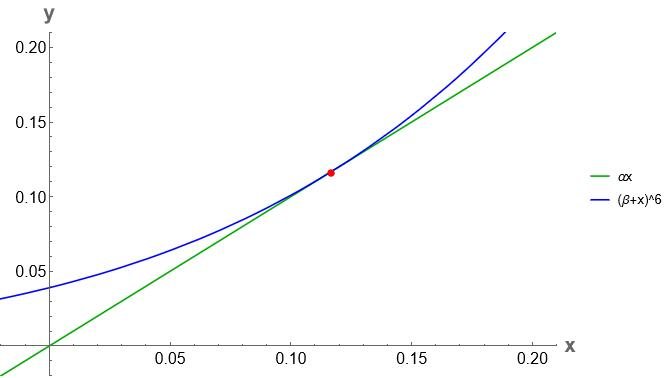
\includegraphics[width=0.77\textwidth]{images/one_intersection.jpg}
            }

            \subfloat[\(\beta = 0.59\)]{
                \label{mainOver}
                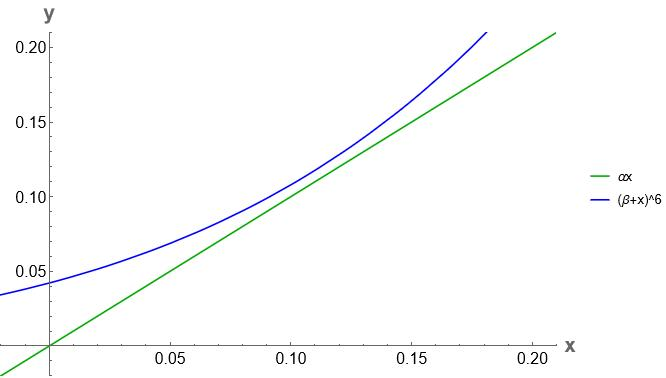
\includegraphics[width=0.77\textwidth]{images/zero_intersection.jpg}
            } 

            \captionsetup{justification=centering}
            \caption{Решения уравнения (\ref{baseEquation}) для разных значений параметра \(\beta\)}
        \end{figure}
        
    \subsection{Временные ряды}

        Для демонстрации поведения системы можно использовать временные ряды. Временной ряд позволяет наглядно показать как с течением времени изменяется численность популяции.

        Далее рассмотрим подробнее основные типичные ситуации. Для этого давайте зафиксируем параметр следующим образом: \(\beta = 0.56\). 

        На рисунке \ref{time_series_b_0_56} мы видим, что временные ряды, которые начинаются в \(x_0 = 0.04\) и в \(x_0 = 1.3\) сходятся к нулю. В биологическом смысле это означает, что популяция с течением времени вымирает.

        А теперь зафиксируем начальную численность популяции на уровне \(x_0 = 0.06\). На рисунке \ref{time_series_b_0_56} видно, что при таких начальных условиях популяция увеличивается до некоторого значения. После достижения которого рост численности популяции прекращается. То есть популяция с течением времени стабилизируется.

        Похожую ситуацию мы можем наблюдать на том же рисунке \ref{time_series_b_0_56} при начальном значении \(x_0 = 0.3\). Значения численности популяции тоже сходятся к устойчивому равновесию. Численность снова стабилизируется.
    
        \begin{figure}
            \centering
            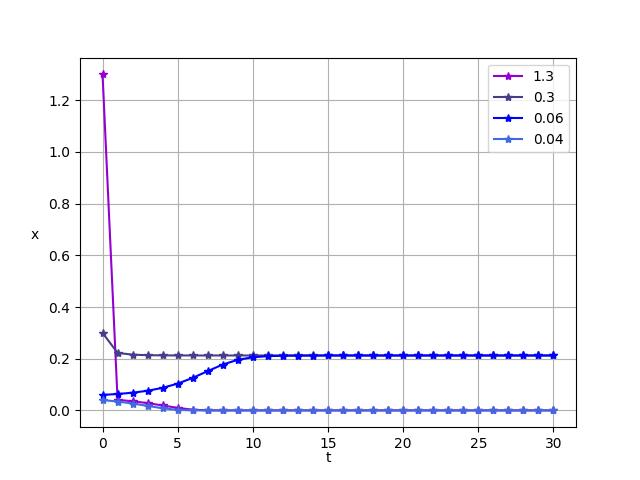
\includegraphics[width=\textwidth]{time_series_b_0_56.jpg}

            \captionsetup{justification=centering}
            \caption{Временные ряды модели (\ref{origin}) для \(\beta = 0.56\) при различных начальных значениях}
            \label{time_series_b_0_56}
        \end{figure}

        Рассмотрим ситуацию, когда \(\beta = 0.4\) и \(x_0 = 0.1\). На рисунке \ref{time_series_x_0_1_b_0_4} можно заметить, что элементы временного ряда принимают два значения. Это соответствуют циклу порядка 2, который можно увидеть на бифуркационной диаграмме, которую можно увидеть на рисунке \ref{bifurcation}.
    
        \begin{figure}
            \centering
            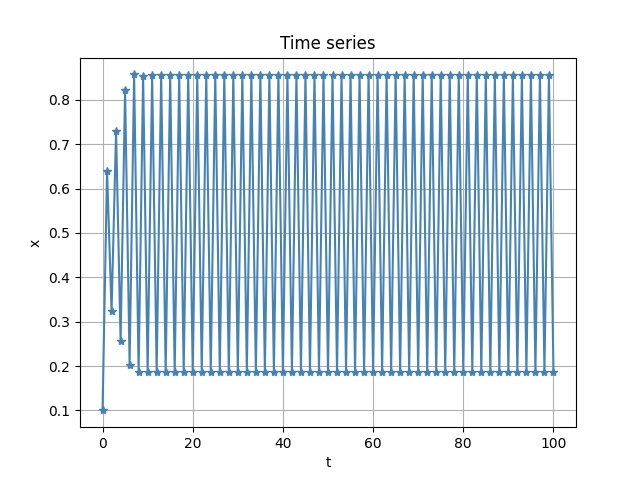
\includegraphics[width=\textwidth]{time_series_x_0_1_b_0_4.jpeg}

            \captionsetup{justification=centering}
            \caption{Временной ряд модели (\ref{origin}) для \(\beta = 0.4\) и \(x_0 = 0.1\)}
            \label{time_series_x_0_1_b_0_4}
        \end{figure}

        Давайте теперь изменим значение параметра: \(\beta = 0.25\). Начальная численность популяции: \(x_0 = 0.1\). На рисунке \ref{time_series_x_0_1_b_0_25} видно, что нет закономерности, по которой меняется численность популяции. Это поведение соответствуют хаосу.
    
        \begin{figure}
            \centering
            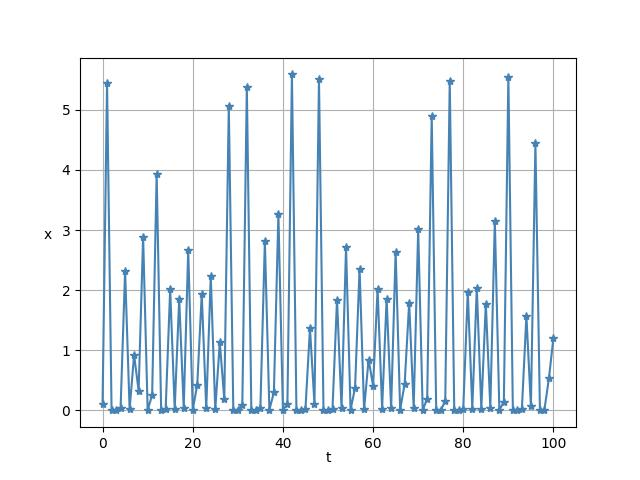
\includegraphics[width=\textwidth]{time_series_x_0_1_b_0_25.jpg}

            \captionsetup{justification=centering}
            \caption{Временной ряд модели (\ref{origin}) для \(\beta = 0.25\) и \(x_0 = 0.1\)}
            \label{time_series_x_0_1_b_0_25}
        \end{figure}

    \subsection{Лестница Ламерея}
    
        Существует также инструмент визуализации решения отображения (\ref{baseEquation}) называемый лестницей Ламерея. Этот метод аналогично временному ряду позволяет иллюстрировать то, как изменяется численность популяции с течением времени.
            
        Опять же рассмотрим подробнее основные типичные ситуации. Для этого зафиксируем параметр: \(\beta = 0.56\). 
    
        \begin{figure}
            \centering
            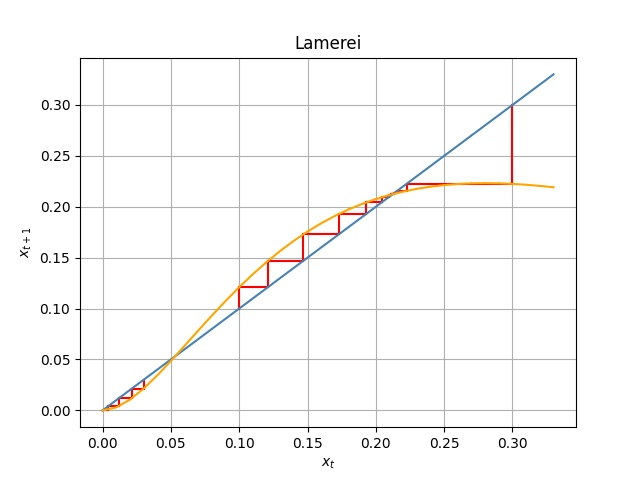
\includegraphics[width=\textwidth]{lamerei_b_0_56.jpg}
    
            \captionsetup{justification=centering}
            \caption{Лестница Ламерея модели (\ref{origin}) для \(\beta = 0.56\) и \(x_0 = 0.03\), \(x_0 = 0.1\) и \(x_0 = 0.3\)}
            \label{lamerei_b_0_56}
        \end{figure}
    
        Давайте зафиксируем начальную численность популяции \(x_0 = 0.03\). На рисунке \ref{lamerei_b_0_56} мы видим, что траектория сходится к нулю. В биологическом смысле это означает, что популяция с течением времени вымирает.
    
        А теперь зафиксируем начальную численность популяции на уровне \(x_0 = 0.06\). На рисунке \ref{lamerei_b_0_56} видно, что при таких начальных условиях численность популяции сходится к \(x \approx 0.21\).
            
        Очень похожую ситуацию мы можем наблюдать на рисунке \ref{lamerei_b_0_56}. Такой график построен при начальном значении \(x_0 = 0.3\). Значения численности популяции тоже сходятся к устойчивому равновесию. Численность снова стабилизируется.
            
        Теперь рассмотрим ситуацию, когда начальная численность популяции очень большая. Такая ситуация изображена на рисунках \ref{lamerei_x_1_3_b_0_56} и \ref{lamerei2_x_1_3_b_0_56}. Мы видим, что популяция вымирает.

        \begin{figure}
            \centering
            \subfloat[Общий вид лестницы Ламерея]{
                \label{lamerei_x_1_3_b_0_56}
                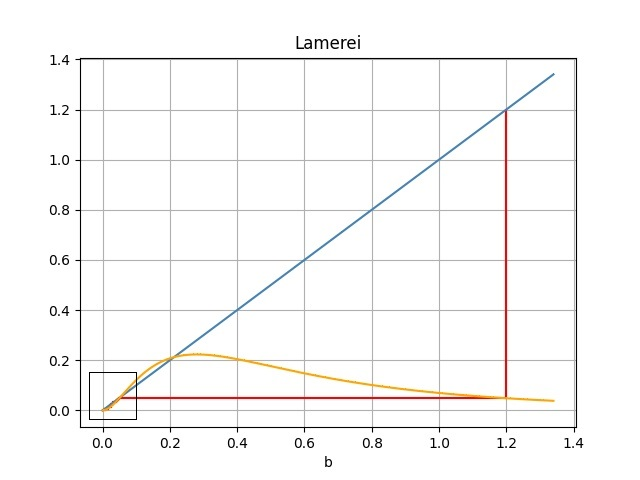
\includegraphics[width=0.9\textwidth]{lamerei_x_1_3_b_0_56.jpg}
            }

            \subfloat[Дополнение к \ref{lamerei_x_1_3_b_0_56}]{
                \label{lamerei2_x_1_3_b_0_56}
                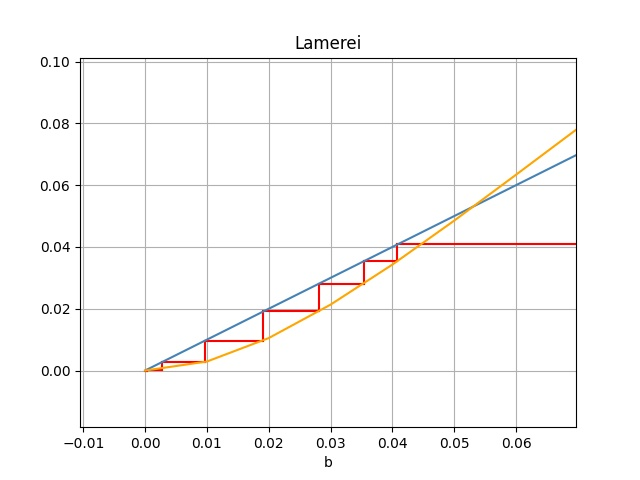
\includegraphics[width=0.9\textwidth]{lamerei2_x_1_3_b_0_56.jpg}
            }

            \captionsetup{justification=centering}
            \caption{Лестница Ламерея модели (\ref{origin}) для \(\beta = 0.56\) и \(x_0 = 1.3\)}
        \end{figure}

        Таким образом, кроме маленького порогового значения численности популяции существует еще и большое значение, задающие интервал существования популяции. Вне этого интервала популяция вымирает. 

    \subsection{Бифуркционная диаграмма}    

        Для визуализации аттракторов при изменении бифуркационного параметра системы строится бифуркационная диаграмма. Бифуркционная диаграмма для модели (\ref{origin}) при \(\alpha = 1\) представлена на рисунке \ref{bifurcation}.

        \begin{figure}
            \centering
            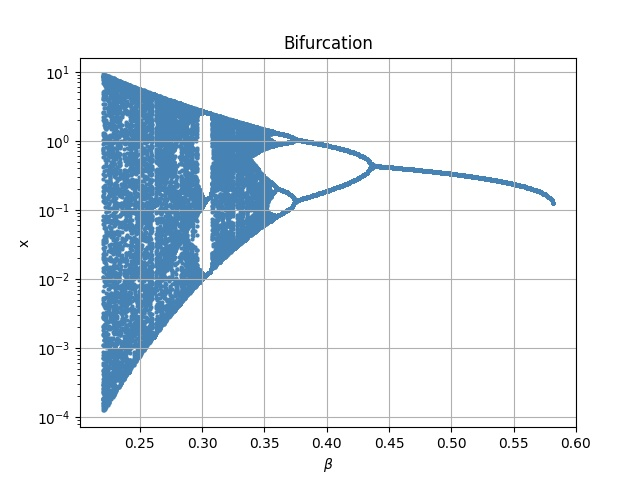
\includegraphics[width=\textwidth]{bifurcation.jpg}

            \captionsetup{justification=centering}
            \caption{Бифуркационная диаграмма модели \ref{origin}}
            \label{bifurcation}
        \end{figure}

        Бифуркационная диаграмма показывает в каком диапазоне изменяется численность популяции при конкретном значении параметра \(\beta\).

        Мы видим, что при \(\beta \in [0.44; 0.56]\) --- аттрактором модели (\ref{origin}) является равновесие. Затем происходит удвоение периода и при \(\beta \in [0.37; 0.44]\) видно, что аттрактором является цикл периода 2. На диапазоне \(\beta \in [0.36; 0.37]\) аттрактором является цикл периода 4. И т.д.
        
        Рассмотренные выше интервалы диапазона значений \(\beta\) являются интервалами структурной устойчивости. При дальнейшем уменьшении значения параметра \(\beta\) зона каждого аттрактора становится все меньше и меньше. 
        
        В модели реализуется каскад бифуркаций удвоения периода, приводящий к хаосу \cite[стр. 33]{elementsOfNonlinearDynamic}. Когда наступает хаос, становится невозможным предсказание значения численности популяции в некоторый момент времени при известном начальном значении.
        
        \begin{figure}
            \centering
            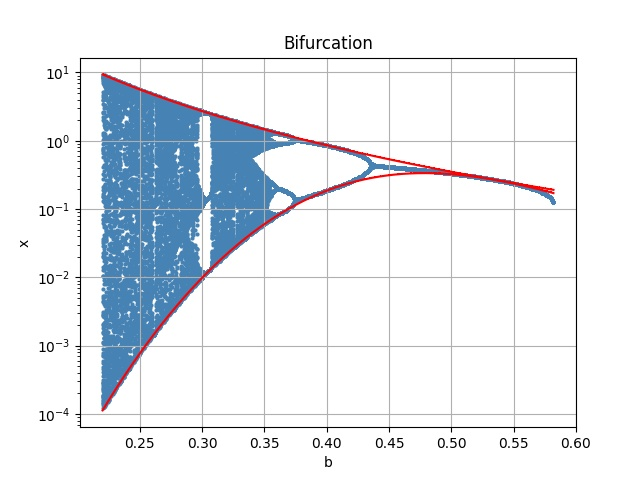
\includegraphics[width=\textwidth]{bifurcation_chaos.jpg}

            \captionsetup{justification=centering}
            \caption{Бифуркационная диаграмма модели (\ref{origin}) --- синим представлены аттракторы модели, красным --- критические линии }
            \label{bifurcation_chaos}
        \end{figure}
        
        Также на бифуркационную диаграмму можно нанести линии, которые показывают границы хаоса, циклов и части равновесия, опираясь на теорию критических точек \cite{nonsmoothOneDimensionalMapsSomeBasicConceptsAndDefinitions}. Такое можно увидеть на рисунке \ref{bifurcation_chaos}. Также можно заметить, что численность популяции на участке хаоса и циклов не выходит за эти границы.
        
        \begin{figure}
            \centering
            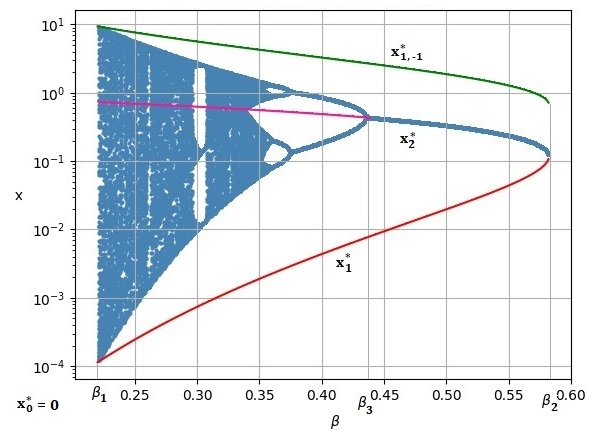
\includegraphics[width=\textwidth]{bifurcation_attract.jpg}

            \captionsetup{justification=centering}
            \caption{Бифуркационная диаграмма модели (\ref{origin}) с равновесиями и образом равновесия \(x_1^*\) }
            \label{bifurcation_attractor}
        \end{figure}

        На рисунке \ref{bifurcation_attractor} изображена бифуркационная диаграмма, равновесия и прообраз неустойчивого равновесия.

        Заметим, что на интервале от \(\beta_3 \approx 0.44\) до \(\beta_2 \approx 0.58\) устойчивое равновесие является аттрактором \cite{elementsOfNonlinearDynamic}.

        Если начальное значение находится в интервале от \(x_1^*\) до \(x_{1, -1}^*\), то траектория сойдется на равновесие \(x_2^*\). В случае, если траектория начинается за пределом этого интервала, то она сойдется на нулевое равновесие.

        Такую ситуацию мы также можем наблюдать при построении временных рядов. На рисунке \ref{time_series_b_0_56} можно увидеть, что если начальное значение \(x_0 = 0.04\) или \(x_0 = 1.3\), то численность популяции сойдется на нулевое равновесие. Эти значения \(x_0\) лежат вне интервала от \(x_1^*\) до \(x_{1, -1}^*\).

        Рассмотрим временные ряды, которые в качестве начальных значений принимают \(x_0 = 0.06\) и \(x_0 = 0.3\). Такие временные ряды сходятся к значению \(x_2^*\), потому что эти значения лежат в бассейне притяжения.

        Исходя из вышесказанного, можно сделать вывод о том, что равновесия \(x_0^*\) и \(x_2^*\) являются устойчивыми, а равновесие \(x_1^*\) --- неустойчивым.

    \subsection{Показатель Ляпунова}    

        Для определения устойчивости аттракторов часто используется показатель Ляпунова. Зависимость этого показателя для аттракторов модели (\ref{origin}) представлена на рисунке \ref{lyapunov}. 

        \begin{figure}
            \centering
            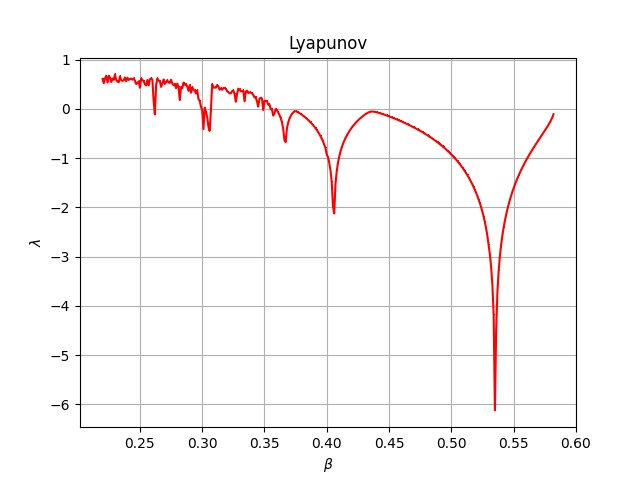
\includegraphics[width=\textwidth]{lyapunov.jpg}

            \captionsetup{justification=centering}
            \caption{Показатель Ляпунова для модели (\ref{origin})}
            \label{lyapunov}
        \end{figure}

        На этом графике мы видим, что точки, где график показателя Ляпунова касается нуля точно соответствуют бифуркционным значениям, которые можно наблюдать на бифуркационной диаграмме представленной на рисунке \ref{bifurcation}.

    \subsection{Карта режимов}

        Карта режимов, представленная на рисунке \ref{regimeMap}, позволяет показать возникающие динамические режимы системы при определенных значениях параметров \(\alpha\) и \(\beta\).

        Можно заметить, что при любом значении параметра \(\alpha\) существует цикл периода  2. Чем меньше параметр \(\alpha\), тем меньше интервал значений параметра \(\beta\), при котором такой цикл существует.

        \begin{figure}
            \centering
            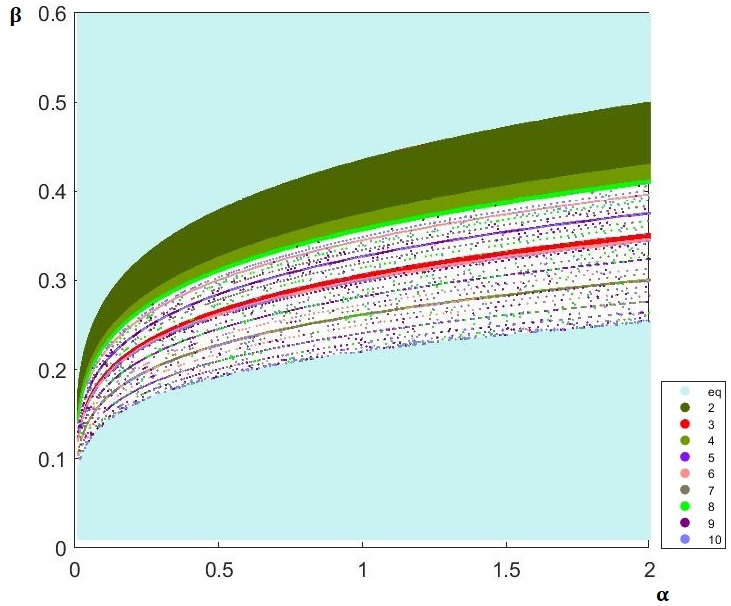
\includegraphics[width=\textwidth]{regime_map.jpg}

            \captionsetup{justification=centering}
            \caption{Карта режимов модели (\ref{origin})}
            \label{regimeMap}
        \end{figure}